The Ascent interface and capabilities are centered around five uses uses:
transforming data, creating images, capturing data, answering questions,
and adpative actions.
%
%
Pipelines describe how to transform data from one form to another.
%
Scenes describe how to render images.
%
Extracts describe how to get data out of Ascent.
%
Queries describe what questions to answer.
%
Triggers decribe conditions, that when satisfied, execute analysis.
%
Ascent refers to these high-level concepts as \textbf{actions},
i.e., tasks to execute in situ.
In this section, we will go over Ascent's abstractions and capabilities.

\fix{I feel like this section should take the following form:
1) what the concept is and 2) what are our current capabilties}

\subsubsection{Pipelines}
Pipelines allows users to describe a series of data transformations, also known as
filters, to execute on simulation data.
%
Figure~\ref{img:pipelines} shows two examples of pipelines.
%
Pipeline \#1 creates contours from a simulation field, and pipeline \#2
thresholds cells that are within a scalar range then applies a clipping operation.
%
In Ascent, users can define as many pipelines as needed.
%
The default source of pipelines, and all other actions, is the data
published by the simulation, but all actions can consume the resutls
of declared pipelines, including other pipelines.

\begin{figure}
\centering
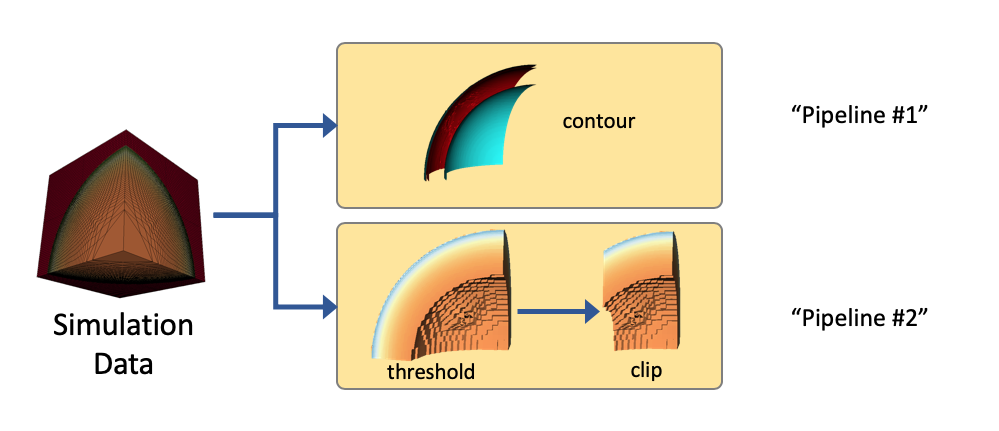
\includegraphics[width=0.6\textwidth]{images/pipelines}
\caption{\label{img:pipelines} Examples pipelines that transforms simulation data via visualization operators.}
\end{figure}

\subsubsection{Scenes}
Scenes allow users to specify how images are rendered.
%
Each scene consists of one or more plots, and Ascent supports volume,
pseudocolor, and mesh plots.
%
Plot types contain parameters such scalar fields, color tables, and scalar ranges,
in addition to the name of the pipeline to consume.
%
Scenes also can contain zero or more \textit{renders}, which contain
camera specifications, image dimensions, background and
forground colors, annotation controls.
%
Ascent creates a default camera based on bounding box of the data set and
is always facing the data set.
%
Renders inherit the default camera parameters, which simplifies creating
cameras that actually looks at the data set.
%
Ascent also provides simple controls to rotate the camera on the
sphere circumscribing the data set, although the user is free to set all
camera parameters explicitly.
%
Additionally, scenes can create Cinema~\cite{AhrensCinema} databases that
create a large set of images that can be explored after the simulation.

\subsubsection{Extracts}
Extracts are an escape hatch in Ascent that enables data to be sent
outside of Ascent.
%
Extracts can be as simple a saving data to HDF5 files or can be a gateway
to a larger workflow (e.g., ADIOS).
%
Ascent supports connections to the Python ecosystem through the Python and
Jupyter extracts~\cite{CyrusISAV}.
%
Python extracts execute custom analysis code provided by the user, and the
Jupyter extracts allow for incoming Jupyter notebooks connnections from a web
browser.

Jupyter notebooks is a promising direction for in situ.
%
One of in situ's greatest weaknesses is the it's reliance on a priori
knowledge, and one strategy to mitagate this weakness is interactivity.
%
Through the Jupyter notebook interface, users can pause a running simulation
and interact with the data.
%
Additionally, Jupyter widgets enable fast prototyping of domain specific
GUIs.

\fix{Cyrus add more wisdom and python stuff.}

\subsubsection{Queries}
\label{action_queries}
Queries in Ascent allow users to ask questions about simulation data,
or data from pipelines, through a Python like language.
%
Queries provide access to data summarization functions and access to the
current state of the simulation..
%
Examples include min-max queries, statistics, cell locations,
and probability distributions.
%
Queries are executed each time Ascent is called, and the resulting time
history can be saved, accessed by the simulation, or accessed in other
expressions.

Queries can be as simple as calling a function that returns the current simulation cycle
and storing it into a variable.
%
More complex queries can calculate the amount of entropy of a field.
%
The expression language that backs queries can perform math operations,
call functions, and conditionals.
%
Since queries are stored into named identifiers, subsequent queires
can build on the results of other queries, allowing for complex combinations.

%Listing~\ref{simple_query} shows the declaration of a query that returns
%the current simulation cycle and stores it into a variable identifier \textit{cycle},
%and Listing~\ref{complex_query} shows a more complex example of a query that
%calculates the entropy of a simulation field.
%\begin{lstlisting}[language=Python,caption={Examples of querying the simulation cycle}, label={simple_query}]
%# add a simple query expression (q1)
%queries["q1/params/expression"] = "cycle()"
%queries["q1/params/name"] = "cycle"
%\end{lstlisting}
%

%
%
%\begin{lstlisting}[language=Python,caption={A more complex example of queries in Ascent}, label={complex_query}]
%# add a more complex query expression (q2)
%queries["q2/params/expression"] = "entropy(histogram(field('gyre'), num_bins=128))"
%queries["q2/params/name"] = "entropy_of_gyre"
%\end{lstlisting}

\subsubsection{Triggers}
Traditional in situ actions execute every $X$ simulation cycles, this presents
two related problems.
%
First, if the analysis is expensive, then the total cost of the action may exceed
what a user is willing to pay, e.g., adding a 50\% overhead on top of the simulation.
%
Second, if the analysis called infrequently, then the feature or event that the analysis is
trying to capture could easily be missed.
%
Triggers address these issues by coupling inspection routines with analysis, and a
potentially costly analysis only executes when user defined precondition is met.
%
Ideally, inpection routines are cheap and can be called every cycle, while the analysis
that are ``triggered'' can cost more.

Ascent triggers builds on the queries and expression support introduced in
Section~\ref{action_queries}, and the trigger condition can be any conditional
expression.
%
When the condition evaluates to true, the trigger fires, executing a user provided
set of actions, which can be any Ascent action.
%
Triggers can be use to execute actions for debugging purposes(i.e., saving data to
a file when invalid values are found) or rendering images when a large
change is found(i.e., when the max value of a field exceeds a threshold from the
previous value).
%
When an event can be expressed in these terms, triggers are a powerful tool for
maximizing constrained resources in situ.


